\prefacesection{Text Analytics Using Rapid Miner}

\section*{Business Understanding}

This following sections shall describe the business objectives, the mining objectives, a analysis and plan for the proposed project.

\subsection*{Business Objective}
The objective of this project is to mine unstructured data using Rapid Miner.

\subsection*{Data Mining objective}
\begin{itemize}
	\item The main objective is to mine articles about Machine Learning, Deep Learning and Robotics. 
	\item Web crawling will be implemented to find related text on the topics.
	\item Preprocessing steps shall be put in place in order to produce the most predictive words for modeling.
	\item Multiple clustering and classification models will be used to identify the texts.
\end{itemize}

\subsection*{Project analysis}
% (cost benifit analysis; risk assessment; resouces needed; assumptions)
In terms of a cost benefit analysis, this project deems relatively efficient due to the benefits out weighing the costs. The proposed assignment poses minimal risk as only a few events may delay the production of the project, such as unavailable texts and misclassification, which are very unlikely. The resources required for this project include: The RapidMiner software and all it's operators related to the data mining objective, articles from online resources, 13 documents based on 3 categories and a online word cloud service for visualisation of predictive words or phrases. 

 
\subsection*{Project plan}
There are a number of steps taken in relation to this project.
\begin{itemize}
	\item Initially, Three categories are decided on. Two topics should be relatively similar, and the last on will be unrelated. In this case, they are based on Deep Learning, Machine Learning and robotics.
	\item Thirteen texts are sourced online for each category. Ten shall be used for training datasets and three shall be used for testing. Web crawling will be implemented using RapidMiner for three of those texts. The steps taken will be documented 
	\item These source articles will be downloaded into their respective folders based on their class label.
	\item A word cloud will be creating to visualise the frequently occurring terms.
	\item Preprocessing steps shall be experimented with to compare stemmers, determine which words are predominantly more predictive, apply pruning and comparing accuracy based on different vectors and documenting the results.
	\item Apply two algorithms for clustering and classification and discuss the accuracy of them.
	\item Lastly, an evaluation of the project will be performed, which will assess the overall result in relation with the business objectives. 
\end{itemize}

%%%%%%%%%%%%%%%%%%%%%%%%%%%%%%%%%%%%%%%%%%%%%%%%%%%%%%%%%%%%

\section*{Data Understanding}
%Eliminate common words & stop words
%Eliminate rare words
%Identify phrases

As previously mentioned, thirteen texts have been obtain online according to three categories: machine learning, deep learning and robotics. Additionally, 3 of these texts were sources through the use of web crawling on Rapid Miner using the \textbf{Crawl Web} operator.
In order to obtain a better insight to the commonly occurring word in the files of each category, word clouds were made. As seen in Figure \ref{mlfig}, Figure \ref{dlfig} and Figure \ref{robfig} three word images were made to visualise the frequent terms. The larger the word appears in the image, the more often it appears in the documents that have been collected.
For machine learning, it is clear that the terms \textbf{knn}, \textbf{training}, \textbf{decision tree}, \textbf{naive bayes} and \textbf{classification}.

\begin{figure}[ht]
	\begin{center}
		\advance\leftskip-3cm
		\advance\rightskip-3cm
		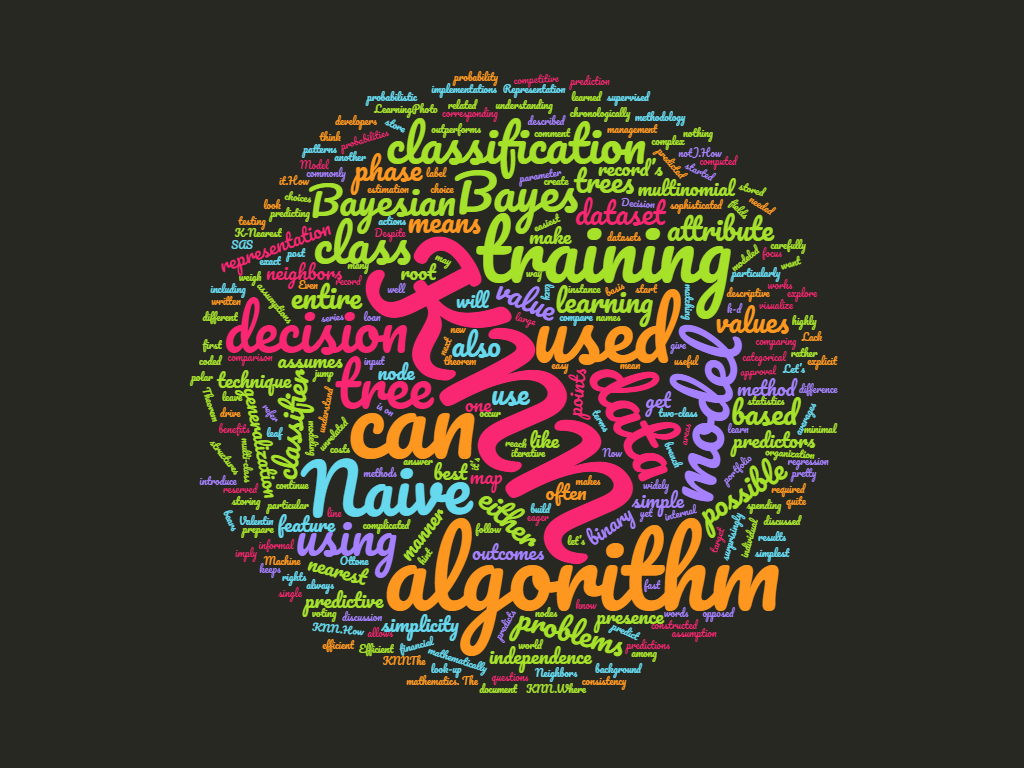
\includegraphics[keepaspectratio=true,scale=0.4]{__resources/machine_learning.png}
		\caption{Word cloud for the machine learning category}
		\label{mlfig}
	\end{center}
\end{figure}

\newpage

A more concise description of deep learning can be seen in Figure 2. Although the two categories are related, these terms seem to focus more so on words like \textbf{networks}, \textbf{neural}, \textbf{CNN's}, \textbf{model} and \textbf{recurrent} to name a few.

\begin{figure}[ht]
	\begin{center}
		\advance\leftskip-3cm
		\advance\rightskip-3cm
		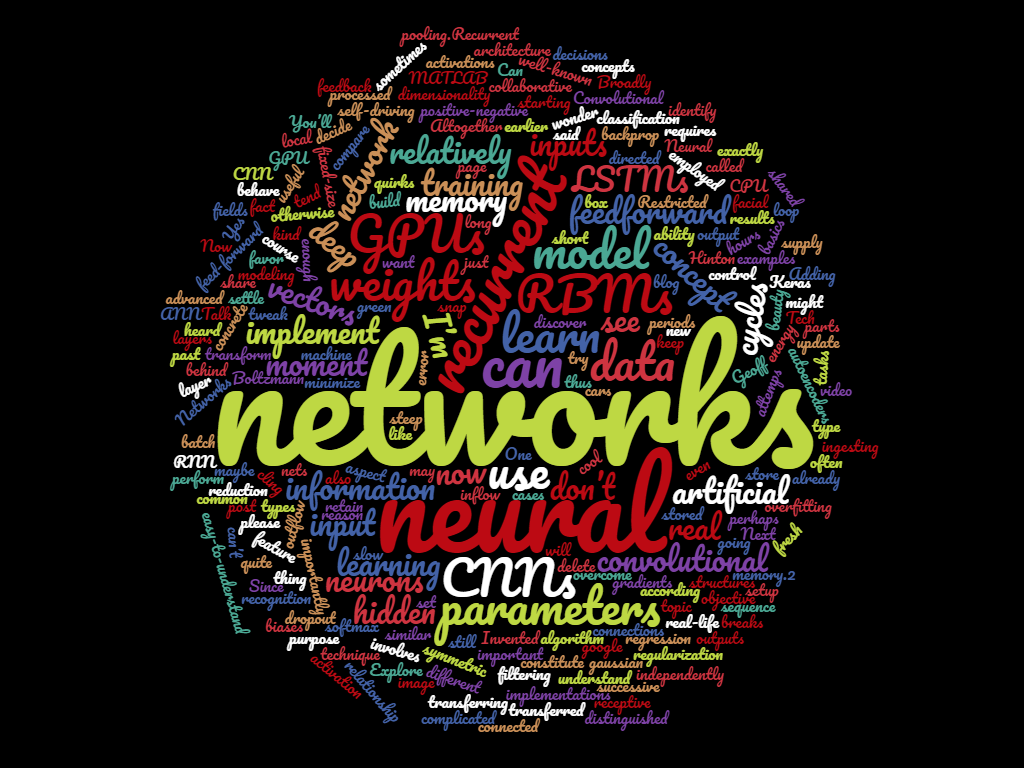
\includegraphics[keepaspectratio=true,scale=0.4]{__resources/deep_learning.png}
		\caption{Word cloud for the deep learning category}
		\label{dlfig}
	\end{center}
\end{figure}

Lastly, we see the terms generated for the robotics category. Evidently, these words are not related to machine learning or deep learning as they share very few words to the documents in the other two categories. The prominent words found here are \textbf{robots}, \textbf{humans} or \textbf{humanoid} and  \textbf{robotics}

\newpage


\begin{figure}[ht]
	\begin{center}
		\advance\leftskip-3cm
		\advance\rightskip-3cm
		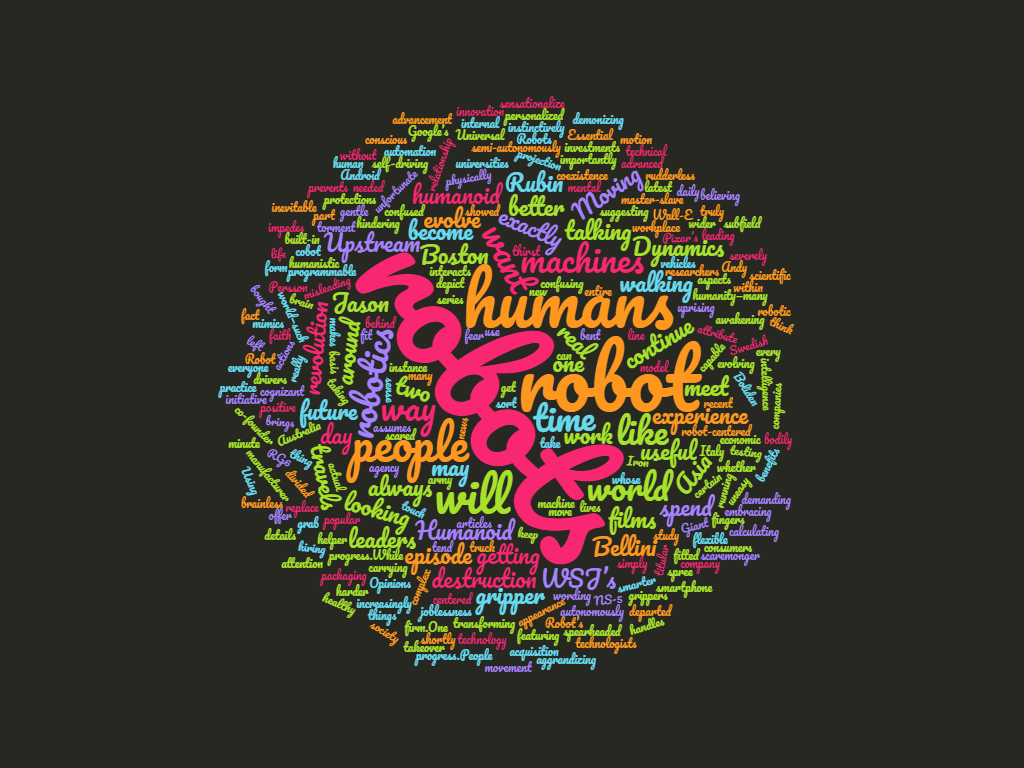
\includegraphics[keepaspectratio=true,scale=0.4]{__resources/robotics.png}
		\caption{Word cloud for the robotics category}
		\label{robfig}
	\end{center}
\end{figure}


Not only do these word clouds help determine predictive words, but also provide certain words that are not useful for the mining objects, also known as stop words. Certain stop words in these figures are "I'm", "thing",  "makes" for example. These words can be ambiguous depending on the sentiment of the article being read or just common English phrases, therefore they should not be included in the working model. \\
Furthermore, potential synonyms can be found in these word clouds. To reduce dimensionality, it is beneficial to specify words that may hold the same meaning. For instance, it can be seen that in the category of robotics, the terms "robot" and "robotics" are in interchangeable, therefore they can be classes as synonyms of one another. Another example of this could be the phrase "neural network" and "ANN", which the latter is an acronym for "neural network" therefore that can also be classed as a synonym.

\newpage

%%%%%%%%%%%%%%%%%%%%%%%%%%%%%%%%%%%%%%%%%%%%%%%%%%%%%%%%%%%%
\newpage
\section*{Data Preparation}
The initial step in the preprocessing phase consists of making a stop word list based on the word clouds. This if followed by the creation of a synonyms lists to group relating terms under the one word. In terms of Rapid Miner processes a number of steps are taken in order to prepare the data for mining. \\ \\

\subsection*{Generating a Bag of Words}
\textbf{Process Documents from Files}: this operator generates word vectors based on text from multiple files, in this case, the texts that have been collected initially.  Within the \textit{Process Documents from Files} operator, a number of other techniques are used to cleanse the data.\\
\textbf{Tokenizing}: to split the text into tokens.\\ \textbf{Transform cases}: which changes everything to the letter case you specify.\\
\textbf{Filter Stopwords (English)}: This operator filters out all the commonly occurring words in the English language which are not useful for text analysis.\\
\textbf{Filter Tokens by Length}: Upon inspection of the word vector that was generated, it was noted that some characters where not filtered by the \textit{Filter Stopwords (by length)} operator as there was still word like "a" and "on" still being seen, therefore this operator was utilized in order to remove these terms. A range between 3 and 25 characters was set for this.\\

After these initial steps, the documents were processed and a number of 690 attributes where generated before pruning. Absolute pruning was implemented. The parameters set for this were between 3 and 15. Many of the attributes were lost as a result of this, with a number of just 45 attributes. In response to this, the parameters where adjusted to be between 2 and 15. This resulted in 155 attributes.\\
The \textbf{Filter Stopwords (Dictionary)} was applied to remove out the words that were unrelated or unimportant in the word clouds. After the stop word filtering, 120 attributes remained. Example of a few of these stop words can be seen in Figure .


\begin{figure}[ht]
	\begin{center}
		\advance\leftskip-3cm
		\advance\rightskip-3cm
		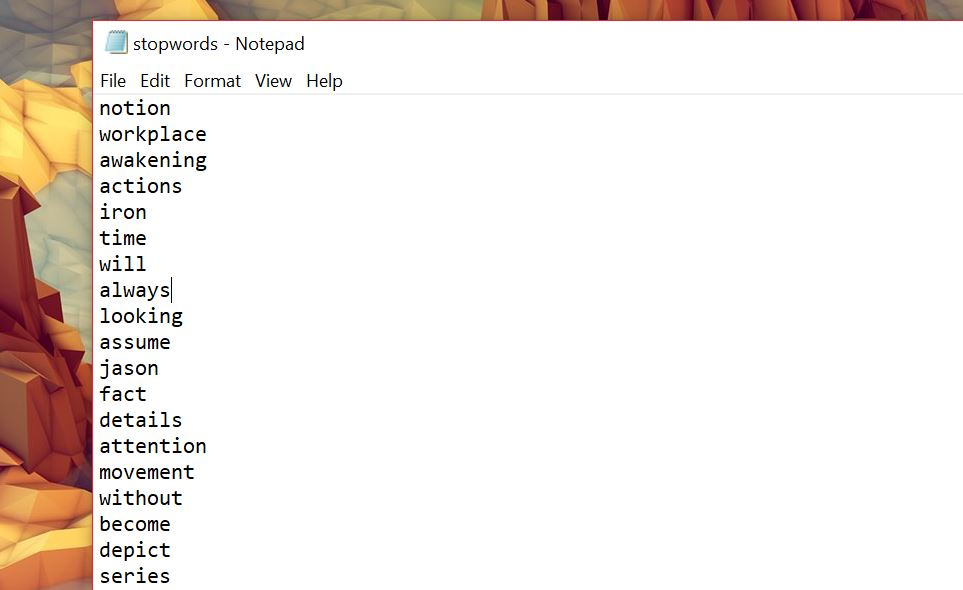
\includegraphics[keepaspectratio=true,scale=0.7]{__resources/stop.JPG}
		\caption{Some of the Dictionary Stop Words}
		\label{stop}
	\end{center}
\end{figure}
\newpage
Following inspection of the terms generated, new stop words were added to the list, bringing it down to 107 attributes. \\ \\
\textbf{Stemming}\\
In order to derive words down to their root stem, two algorithms were utilized, Lovins Stemmer and Port Stemmer. 122 attributes were a result of using Lovins stemmer, reduces the quality as it transforms words like "action" to "act" or completely transforms certain terms into words that do not make any sense, for example: the word "activation" became "activ".

Secondly, Porters stemmer produced 118 attributes, which is a minor improvement as it produced less malformations of worlds. Also to be noticed, it picked up on synonyms of certain words. For example, words like "robotics" and "robot's" all became robot. However, some words were have been completely transformed. Therefore, it is a better approach to apply a stem dictionary. 

A dictionary was created using not only with the words noticed in the word clouds, but the words that appeared in the file processing steps. The application of this list of synonyms reduced the dimensionality to 86 attributes. It can be seen that applying words like "LSTM", "CNN", "network" under a more generalized term such as \textbf{neural-network}, 41 occurrences appear in the document for Deep Learning. 
This trend can be also be seen with terms like "nearest-neighbor" "k-nn" to simply fall under the term \textbf{knn}, which appears 21 times in the documents for machine learning and 1 time in the document for deep learning.
Furthermore, the word "humanoid", a descriptive term that is used in the phrase "humanoid robot", appears entirely within the category of robotics at a cardinality of 13. \\ \\
\begin{figure}[ht]
	\begin{center}
		\advance\leftskip-3cm
		\advance\rightskip-3cm
		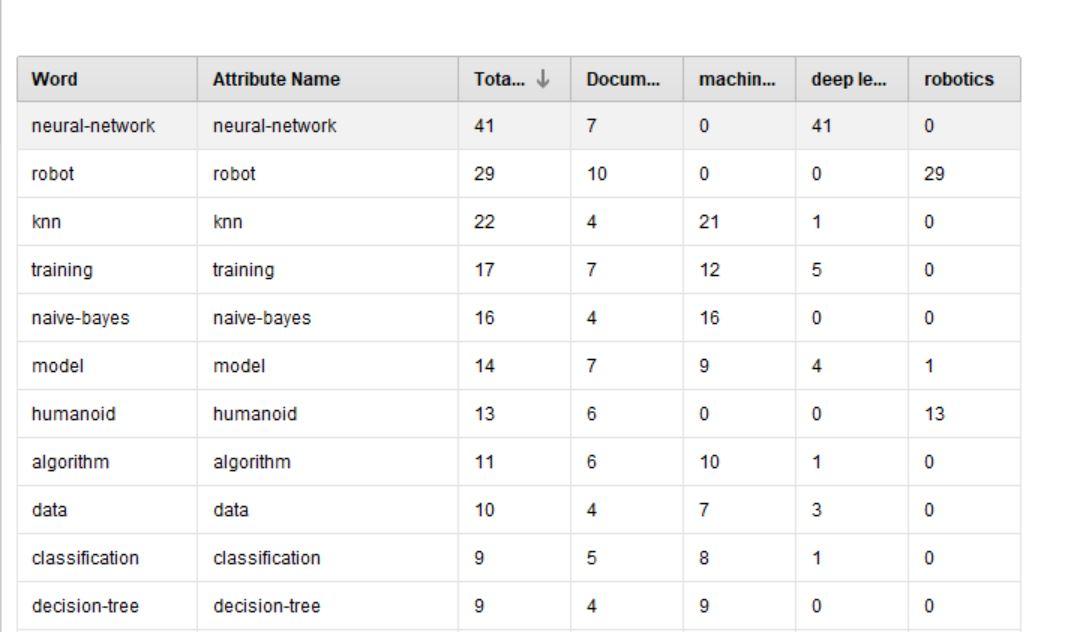
\includegraphics[keepaspectratio=true,scale=0.8]{__resources/1.JPG}
		\caption{Results of Word Generated Using Synonym List}
		\label{stop}
	\end{center}
\end{figure} 
\newpage 

\textbf{Generate N-Grams}\\
Experimentation was conducted on using N-Gram generation instead of tokenizing because of certain combinations of words like "artificial neural network" or "restricted boltzmann machine". Initially, the \textbf{Generate N-Grams (Characters)} operator was used and the length was set to 25 as there are 25 characters in the phrase \textit{artificial neural network}. Upon evaluation it was noted that there were 365 attributes in the dataset, along with certain phrases that did not seem predictive or relevant to the categories of the documents. Therefore N-gram generation will not be used through the remaining phases of this project.


\subsection*{Creating a Document Vector}
The previous section focuses mostly on the terms that appear in the documents. This section will dwell on the cardinality of the terms within the documents. A document vector will be generated, which will be the data for the clustering and classification algorithms to be trained on. Firstly, a cross validation building block with a decision tree operator was added in order test the accuracy of different vector types, in this case: \textbf{Term Occurrence} and \textbf{TD-IDF}. \\ 


\subsubsection*{TD-IDF}
With TD-IDF, using absolute pruning between 2 and 15, an accuracy of 86.67\% was achieved. See Figure 6 for the RapidMiner confusion matrix.

\begin{figure}[ht]
	\begin{center}
		\advance\leftskip-3cm
		\advance\rightskip-3cm
		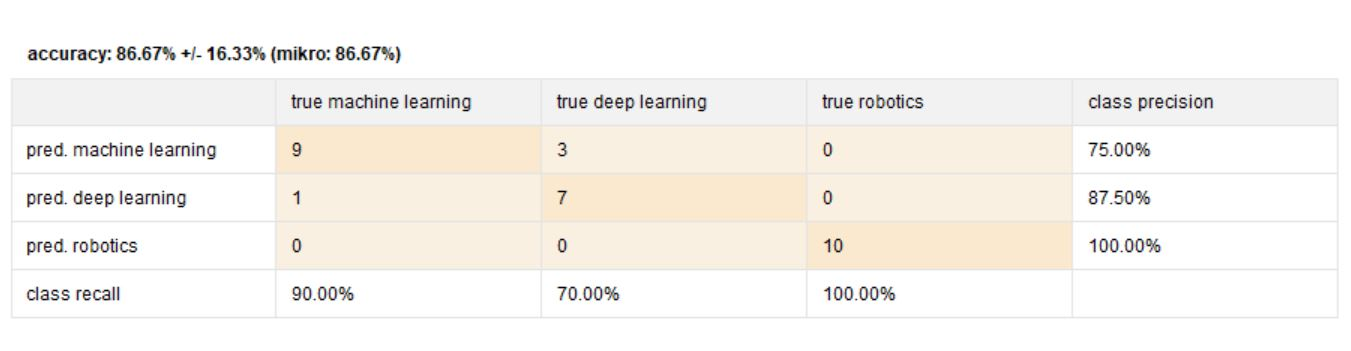
\includegraphics[keepaspectratio=true,scale=0.6]{__resources/tdidf.JPG}
		\caption{Accuracy using }
		\label{stop}
	\end{center}
\end{figure} 
\newpage

Secondly, pruning by rank was applied with a below rank of 0.5 and 0.95. However, this showed pour results as the accuracy only 20.00\% and number of 495 attribute generated.
Percentual Pruning was applied to the model with a prune below percentage of 3.0 and a prune above percentage of 30.0. This resulted in an accuracy of 46.67\%.

\subsubsection*{Term Occurence}
With Term Occurrence, a better score was achieved, with a 90.00\% accuracy which can be seen in Figure 7. This was achieved using absolute pruning with a range between 2 and 15.

\begin{figure}[ht]
	\begin{center}
		\advance\leftskip-3cm
		\advance\rightskip-3cm
		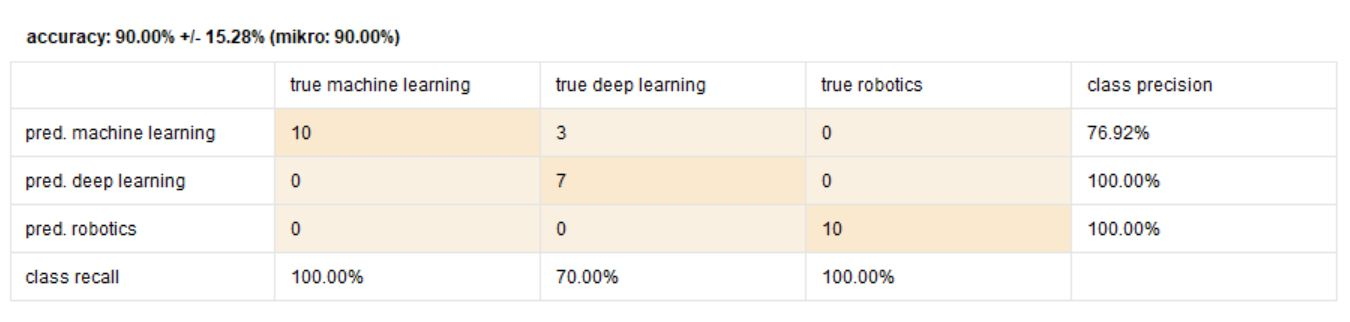
\includegraphics[keepaspectratio=true,scale=0.6]{__resources/to.JPG}
		\caption{Accuracy using }
		\label{stop}
	\end{center}
\end{figure} 

Similar to TD-IDF, the ranking prune method was used with the same metrics, which returned a slightly higher accuracy score of 23.33\%.\\
Overall, it is evident that term occurrence using the absolute pruning method proves to be the most accurate for vector creation. Furthermore, in order to use this data for training when using clustering or classification algorithms, it needs to be saved. Therefore, the \textbf{store} operator is used within the process.


%Generate a document vector based on
%selected concepts (terms and phrases)


%%%%%%%%%%%%%%%%%%%%%%%%%%%%%%%%%%%%%%%%%%%%%%%%%%%%%%%%%%%%
\section*{Modelling}

\subsection*{Modelling techniques}
To test the data that has been prepared two approaches will be taken. Firstly, two clustering algorithms will be used to see if they can identify groups in which the documents reside. It will be evaluated whether or not does the cosine numerical measure improve accuracy of the model and seen whether minimum or maximum linkage is better suited for the dataset that has been generated. Additionally, two classification algorithms applied and evaluated on which returned the most better results on the testing documents.
In terms of algorithms, for clustering K-Means and Agglomerative Clustering algorithms shall be used. For classification, K-NN and naive bays shall be used. 
\subsection*{Clustering}
\subsubsection*{K-Means}
The k-means algorithm was first applied for evaluation. The initial configurations are as follows. K (the amount of clusters) was set to 3, 10 max runs were used, the measurement type was set to numerical and the \textbf{EuclideanDistance} was used as a symmetric distance measurement. The model performs rather poorly, misgrouping some of the documents into the wrong classes, with majority of the documents being grouped into \textit{cluster\_2}. See Figure 8 for a scatter plot of K-means.

\begin{figure}[ht]
	\begin{center}
		\advance\leftskip-3cm
		\advance\rightskip-3cm
		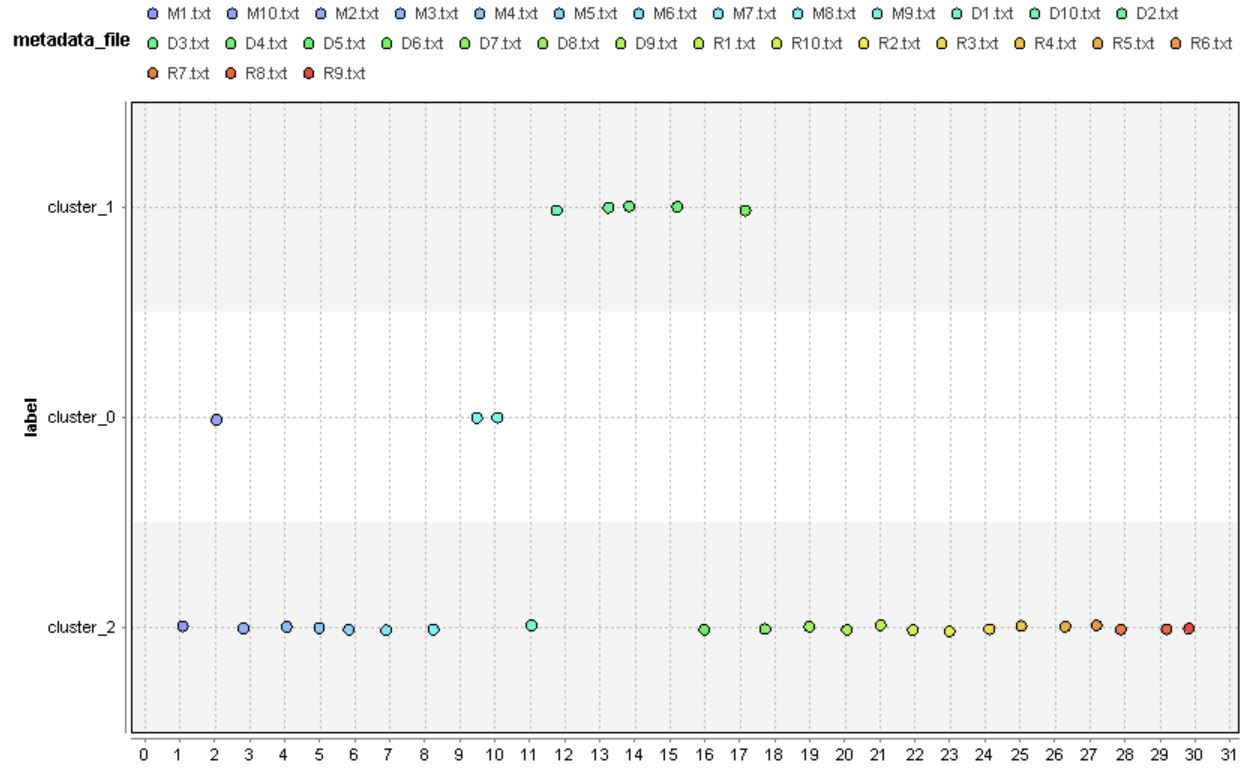
\includegraphics[keepaspectratio=true,scale=0.6]{__resources/kmeans1.JPG}
		\caption{K-means Clustering Scatter Plot}
		\label{stop}
	\end{center}
\end{figure} 

After this the \textbf{CosineSimilarity} asymmetric similarity measure was applied. This improved the performance of the model with majority of the documents being grouped in their respective classes. See Figure 9. for visualisation of improved performance.

\begin{figure}[ht]
	\begin{center}
		\advance\leftskip-3cm
		\advance\rightskip-3cm
		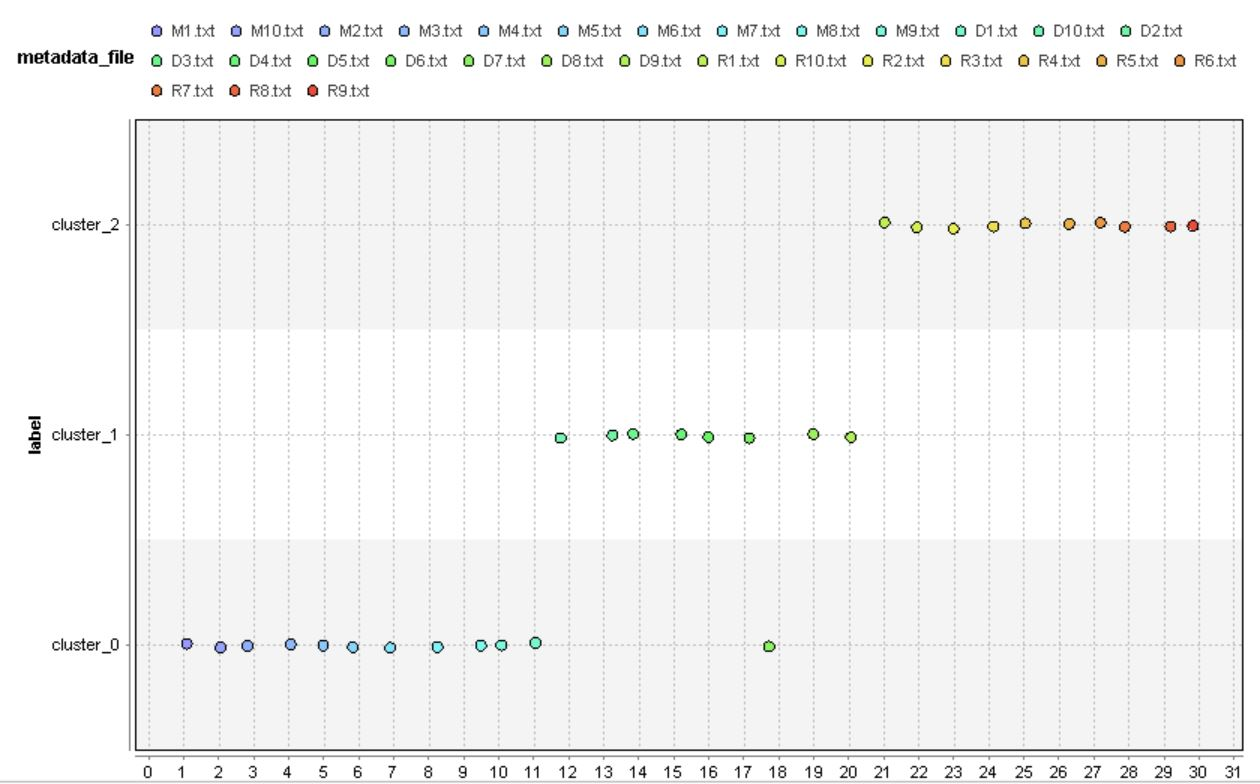
\includegraphics[keepaspectratio=true,scale=0.6]{__resources/kmeans2.JPG}
		\caption{K-means Clustering Scatter Plot Using Cosine Similarity}
		\label{stop}
	\end{center}
\end{figure} 

\subsection*{Agglomerative Clustering}
For agglomerative clustering the parameter configurations are as follows: the measurement type was set to numeric, the measurement was set to \textbf{CosineSimilarity}, the number of clusters is equal to three and the minimum (single) linkage was applied initially. The model performed very well, identifying all the documents into the appropriate clusters.

\begin{figure}[ht]
	\begin{center}
		\advance\leftskip-3cm
		\advance\rightskip-3cm
		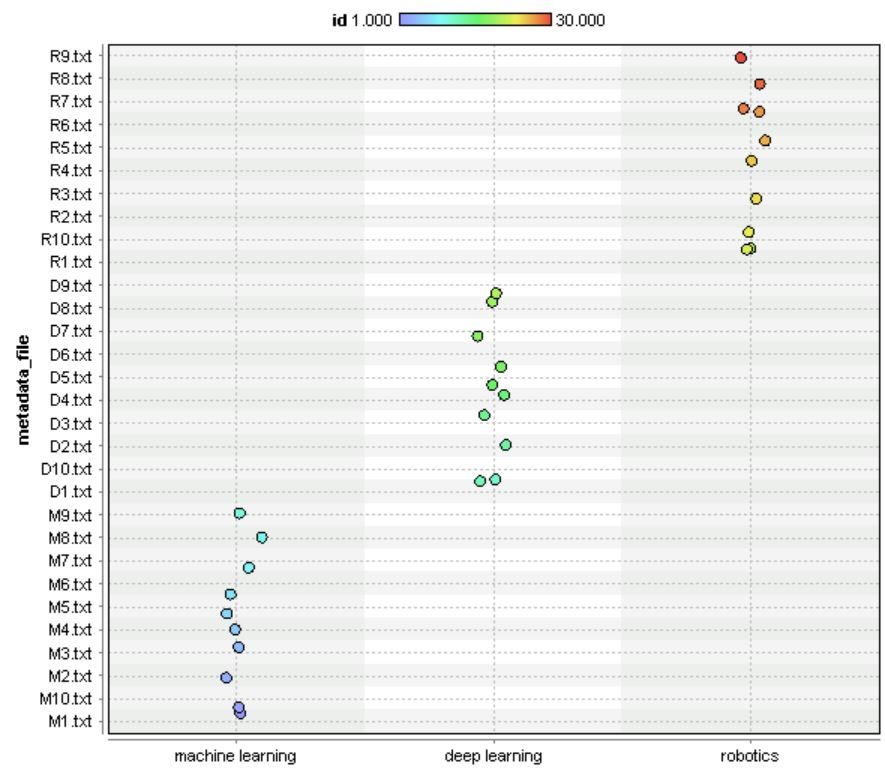
\includegraphics[keepaspectratio=true,scale=0.7]{__resources/agg1.JPG}
		\caption{Agglomerative Clustering Using Minimum Linkage}
		\label{stop}
	\end{center}
\end{figure} 
\newpage

Complete linkage was then applied to the model, this did not make any increase or decrease in performance. However, due to a bug with RapidMiner, the dendrogram was unenviable as it cut off have of the diagram, therefore it is uncertain to comment on which method is more desirable. 



\subsubsection*{Classification}
This section deals with classification of the document vector. Two models shall be used to assess the accuracy. Ideally, a support vector machine would be used, as it is known to be the most accurate of predictive models, but as it only supports a binary class input and we have three, K-NN and Naive Bayes shall be used.
\subsection*{K-NN}
On of the classification algorithms used was K-NN. The reason why this classifier is beneficial is because it requires no training in order to achieve it's function. However, it may require time adjusting parameters to find an optimal point to find the most accuracy.
Firstly, the cross validation operator was used. Within this, K-NN was implemented with \textbf{CosineSimilarity} within a cross validation building block. The model performed relatively well, with a 93.33\% accuracy rate, only misclassifying 2 documents as deep learning.


\begin{figure}[ht]
	\begin{center}
		\advance\leftskip-3cm
		\advance\rightskip-3cm
		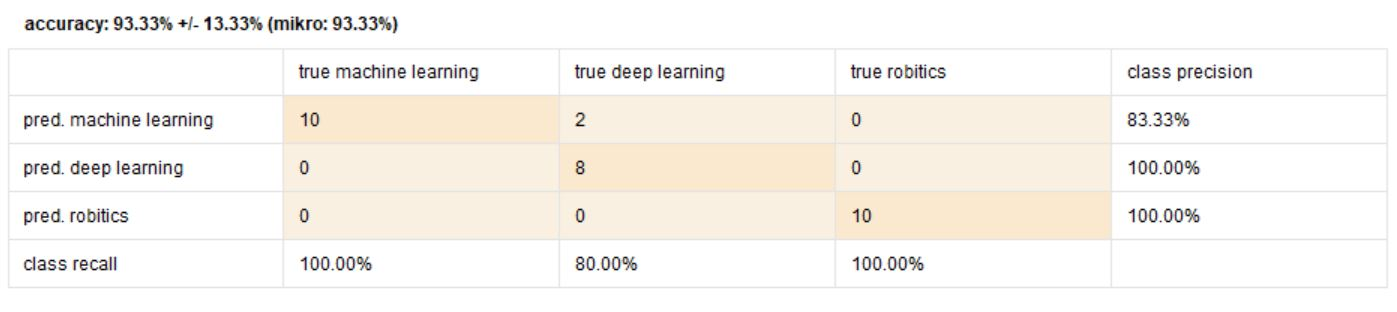
\includegraphics[keepaspectratio=true,scale=0.7]{__resources/knn1.JPG}
		\caption{K-NN Accuracy}
		\label{stop}
	\end{center}
\end{figure} 

This process was repeated numerous times changing the value of K in an incremental manner. This went on until K was equal to 6, where the accuracy decreased until 90.00\%. This drop fluctuated up and down with the accuracy becoming worse gradually. Therefore, the optimal point to keep is at 5. 

\subsection*{Naive Bayes}
Secondly, The Naive Bayes algorithm was utilized. The beneficial factors of this algorithm is that it has minimal training time.   This deems as a good classifier as it received initially 93\% accuracy rate. Upon further explanation with the cross validation parameters, an optimal point was found with the number of folds applied. At three folds for validation, the accuracy was increased to 96.67\%. 

\begin{figure}[ht]
	\begin{center}
		\advance\leftskip-3cm
		\advance\rightskip-3cm
		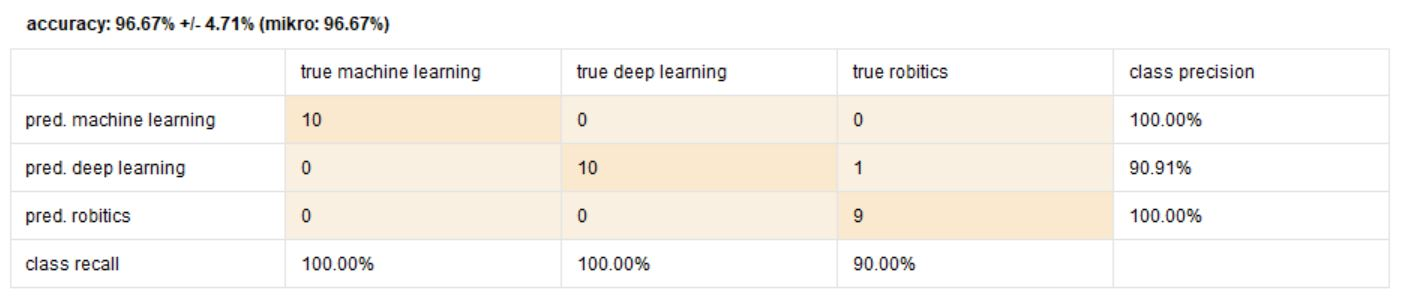
\includegraphics[keepaspectratio=true,scale=0.7]{__resources/bayes1.JPG}
		\caption{Niave Bayes Accuracy}
		\label{stop}
	\end{center}
\end{figure}

\section*{Evaluation}
The following section will review and evaluate the results and performance of the techniques used within this project in respects to the goals of the business and data mining objectives.

\subsection*{Clustering}
\subsubsection*{Subjective Evaluation}
Upon inspection on the clustering techniques applied in the project, it is evident that the agglomerative clustering model accurately grouped the documents into their respective fields, which can be seen in Figure 10.
Additionally, using a parallel plot we can see a high term count for the descriptive terms in their respective clusters, which can be seen below in Figure 13

\begin{figure}[ht]
	\begin{center}
		\advance\leftskip-3cm
		\advance\rightskip-3cm
		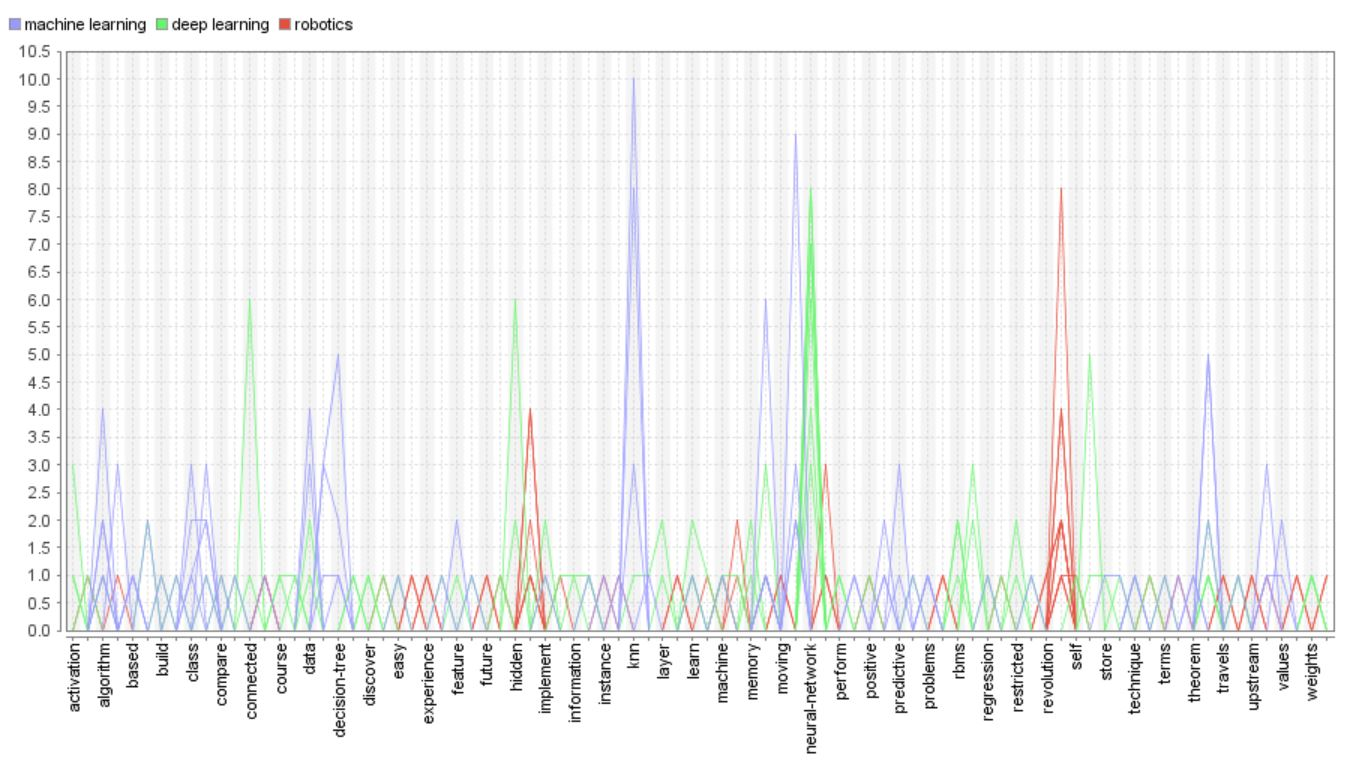
\includegraphics[keepaspectratio=true,scale=0.7]{__resources/cluster-eval.JPG}
		\caption{Parallel Plot For Agglomerative Clustering}
		\label{stop}
	\end{center}
\end{figure}
\newpage

\subsubsection*{Objective Evaluation}
To evaluate the K-Means model, The Davies Bouldin operator will be applied to evaluate the intercluster distance. As can be seen below, the \textbf{Performance (Cluster Distance Performance)} operator was applied. This returned a result: Davies Bouldin: -1.829.

\begin{figure}[ht]
	\begin{center}
		\advance\leftskip-3cm
		\advance\rightskip-3cm
		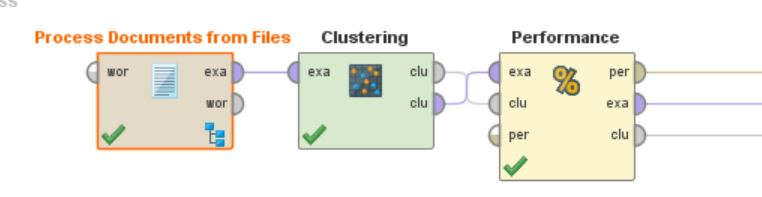
\includegraphics[keepaspectratio=true,scale=0.9]{__resources/db.JPG}
		\caption{Parallel Plot For Agglomerative Clustering}
		\label{stop}
	\end{center}
\end{figure}

\newpage
\subsection*{Classification}
It was desired to apply an ROC to these models but as they don't have a binary class label i was unable to do so. Therefore, the confusion matrices will be used to evaluate their performance.
As can be seen within the figures 11 and 12, the two classifiers gained fairly accurate results, with K-NN having an overall accuracy or 93.33\% and the Naive Bayes model resulting in an accuracy of 96.67\%.

%%%%%%%%%%%%%%%%%%%%%%%%%%%%%%%%%%%%%%%%%%%%%%%%%%%%%%%%%%%%
\section*{Conclusion and Project review}
In conclusion, the business and data mining objective have been met to: mine unstructured data using Rapid Miner, Web crawl for documents on a given category, preprocess the mined data and apply that data to multiple clustering and classification algorithms. 
The models were successful in grouping by category and identifying the classes in which the documents should classed. 


